\documentclass{standalone}
\usepackage{tikz}

\begin{document}

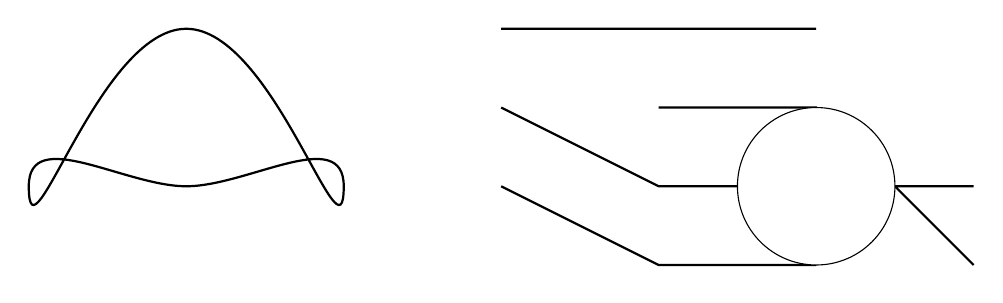
\begin{tikzpicture}[scale=2]

% Define coordinates for the left shape
\coordinate (A) at (-1,0);
\coordinate (B) at (0,0);
\coordinate (C) at (1,0);
\coordinate (D) at (0,1);

% Draw the left shape: a modified curve with circular ends
\draw[thick] (A) to[out=90,in=180] (B)
             to[out=0,in=90] (C)
             to[out=-90,in=0] (D)
             to[out=180,in=-90] (A);

% Define coordinates for the right shape
\coordinate (E) at (3,0);
\coordinate (F) at (4,0);
\coordinate (G) at (5,0);
\coordinate (H) at (4,1);
\coordinate (I) at (3,1);
\coordinate (J) at (2,1);
\coordinate (K) at (2,0);
\coordinate (L) at (3,-0.5);
\coordinate (M) at (4,-0.5);
\coordinate (N) at (5,-0.5);
\coordinate (O) at (4,0.5);
\coordinate (P) at (3,0.5);
\coordinate (Q) at (2,0.5);

% Draw the right shape: a mix of curves and lines with a cut-out circle
\draw[thick] (E) -- (F) -- (G)
             (H) -- (I) -- (J)
             (K) -- (L) -- (M)
             (N) -- (O) -- (P)
             (Q) -- (E);

% Draw the cut-out circle
\filldraw[fill=white, draw=black] (4,0) circle (0.5);

\end{tikzpicture}

\end{document}